\chapter{Практические задания}
\section{Представить следующие списки в виде списочных ячеек:}

'(open close halph)
\begin{figure}[H]
	\centering{
		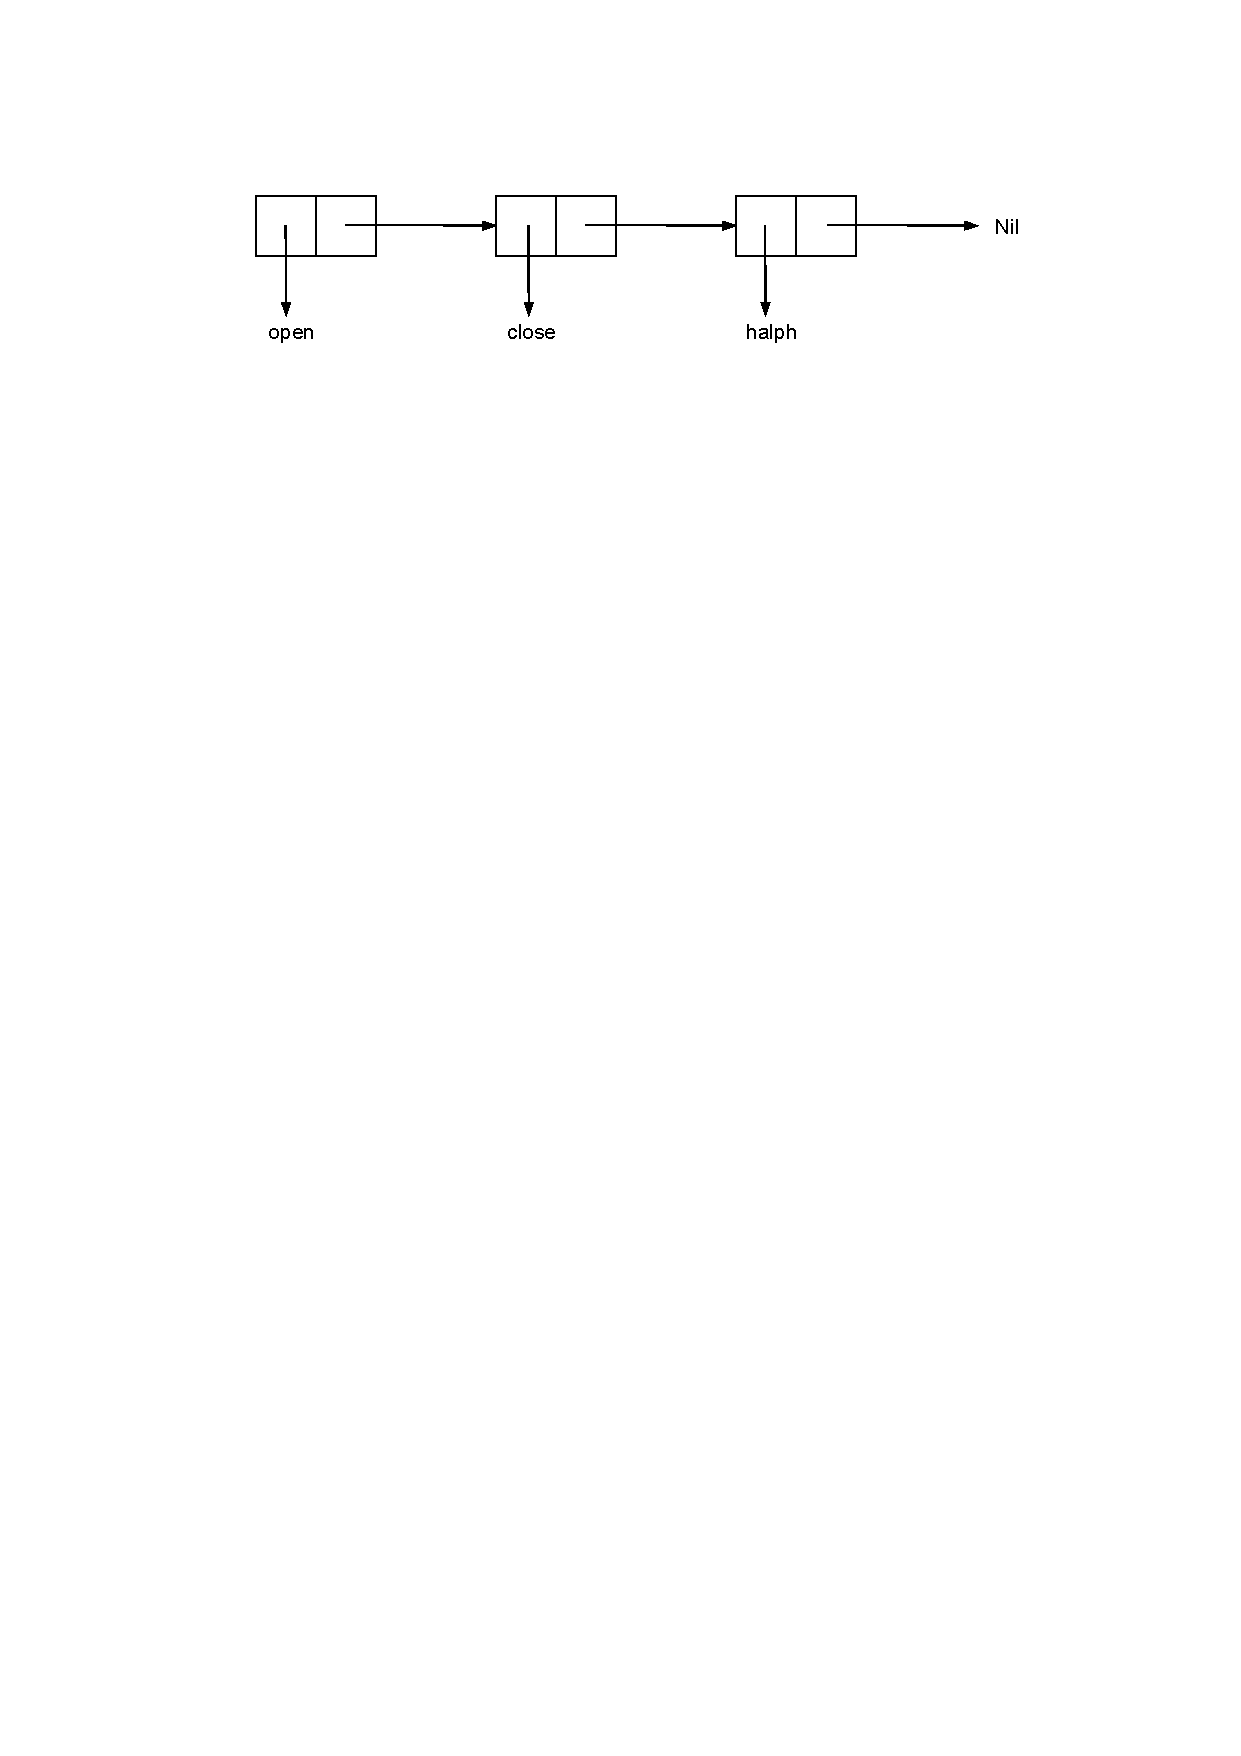
\includegraphics[scale=1]{images/task_1 (1).pdf}}
\end{figure} 

'((open1) (close2) (halph3))
\begin{figure}[H]
	\centering{
		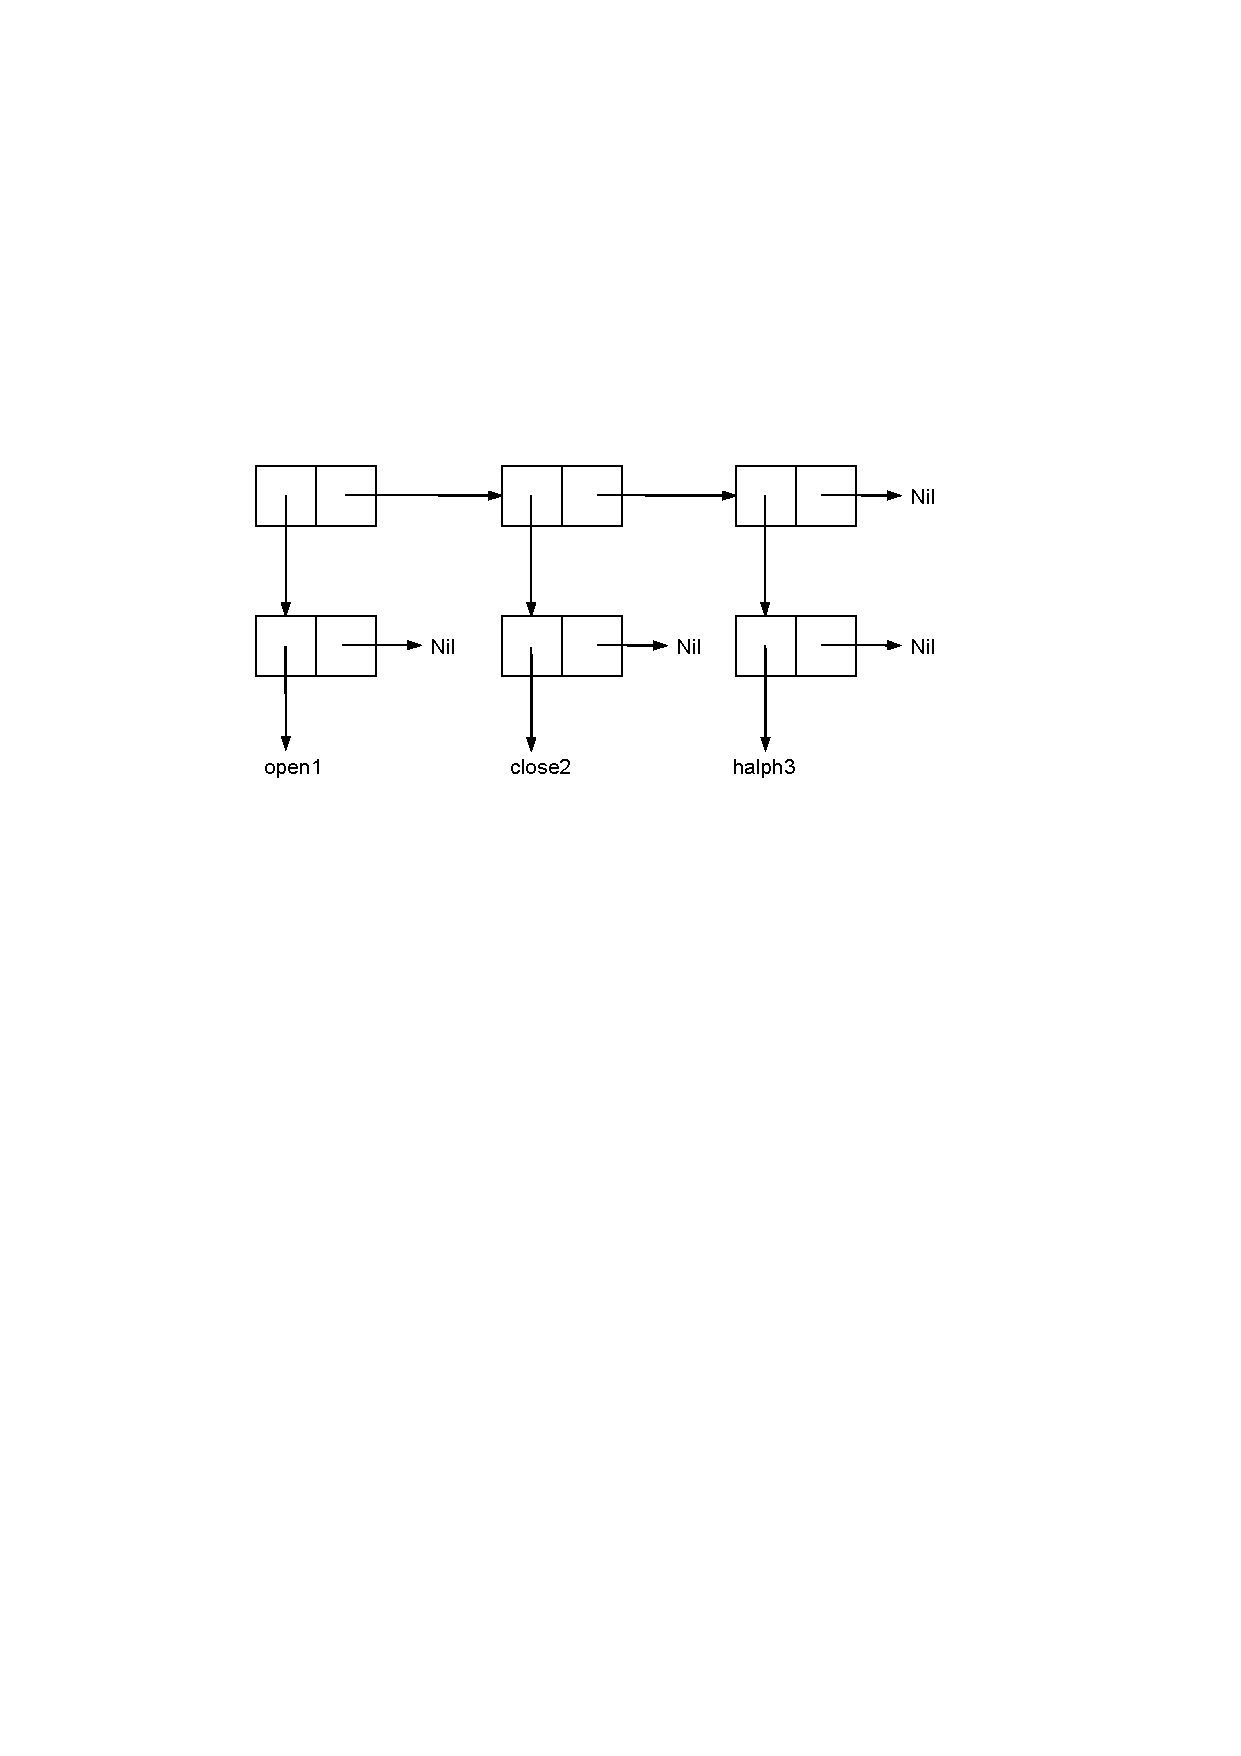
\includegraphics[scale=1]{images/task_1 (2).pdf}}
\end{figure} 

\newpage

'((one) for all (and (me (for you))))
\begin{figure}[H]
	\centering{
		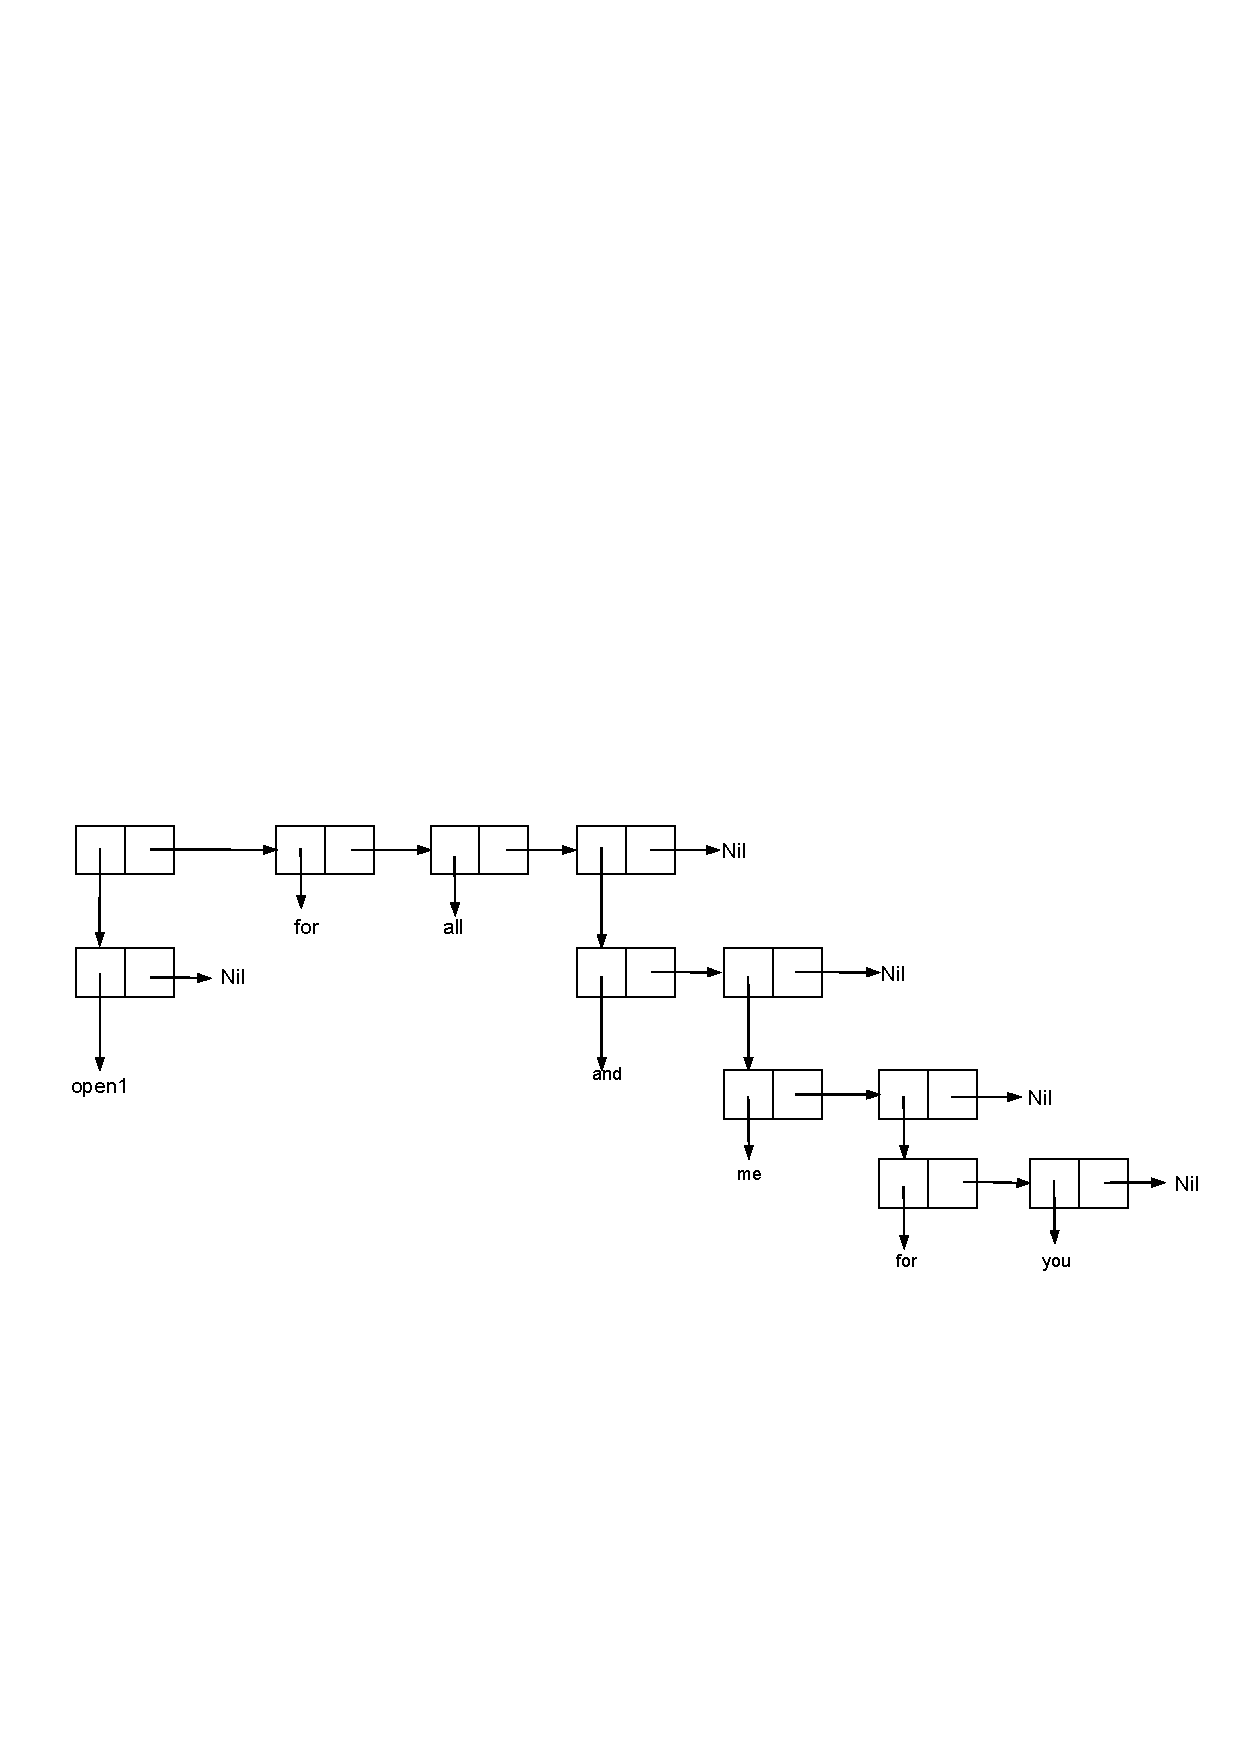
\includegraphics[scale=0.8]{images/task_1 (3).pdf}}
	\end{figure} 

'((TOOL) (call))
\begin{figure}[H]
	\centering{
		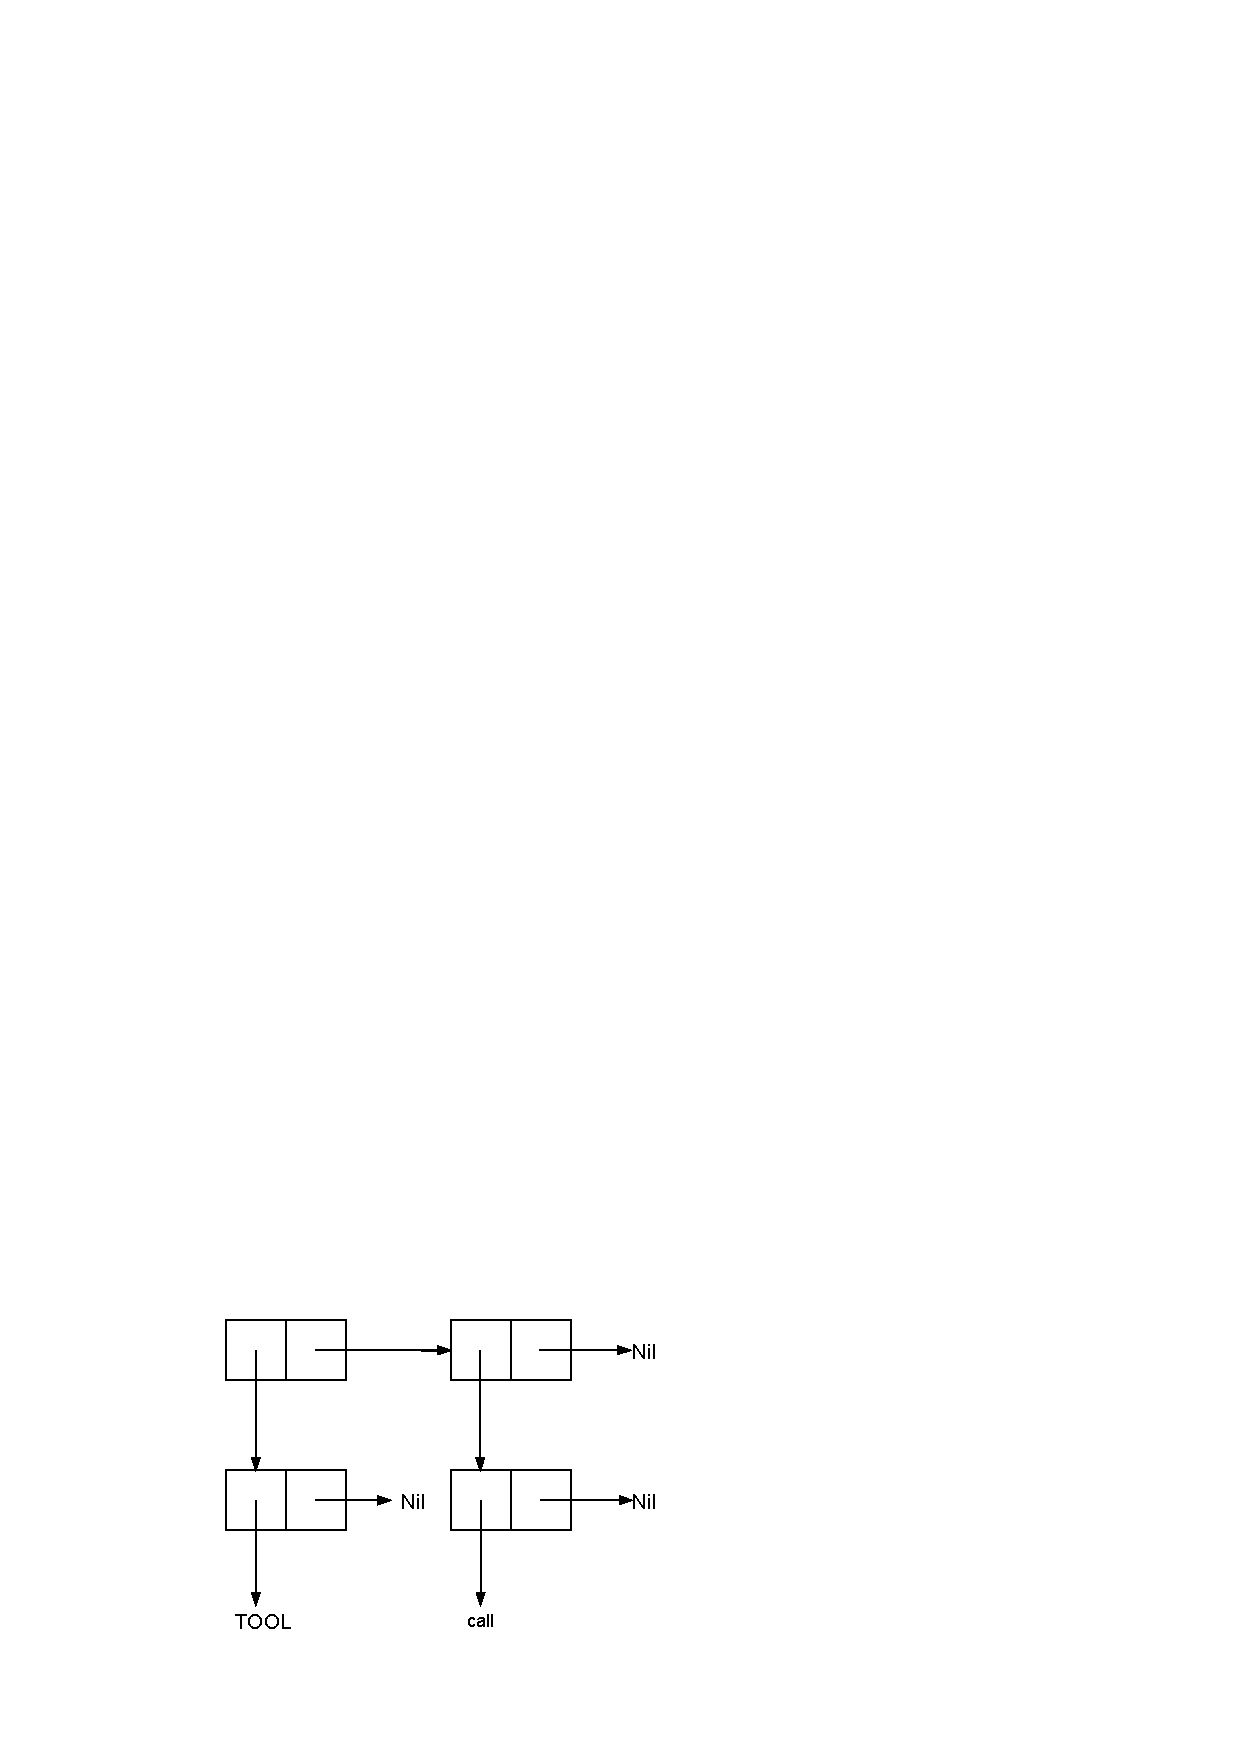
\includegraphics[scale=1]{images/task_1 (4).pdf}}
	\end{figure} 

'((TOOL1) ((call2)) ((sell)))
\begin{figure}[H]
	\centering{
		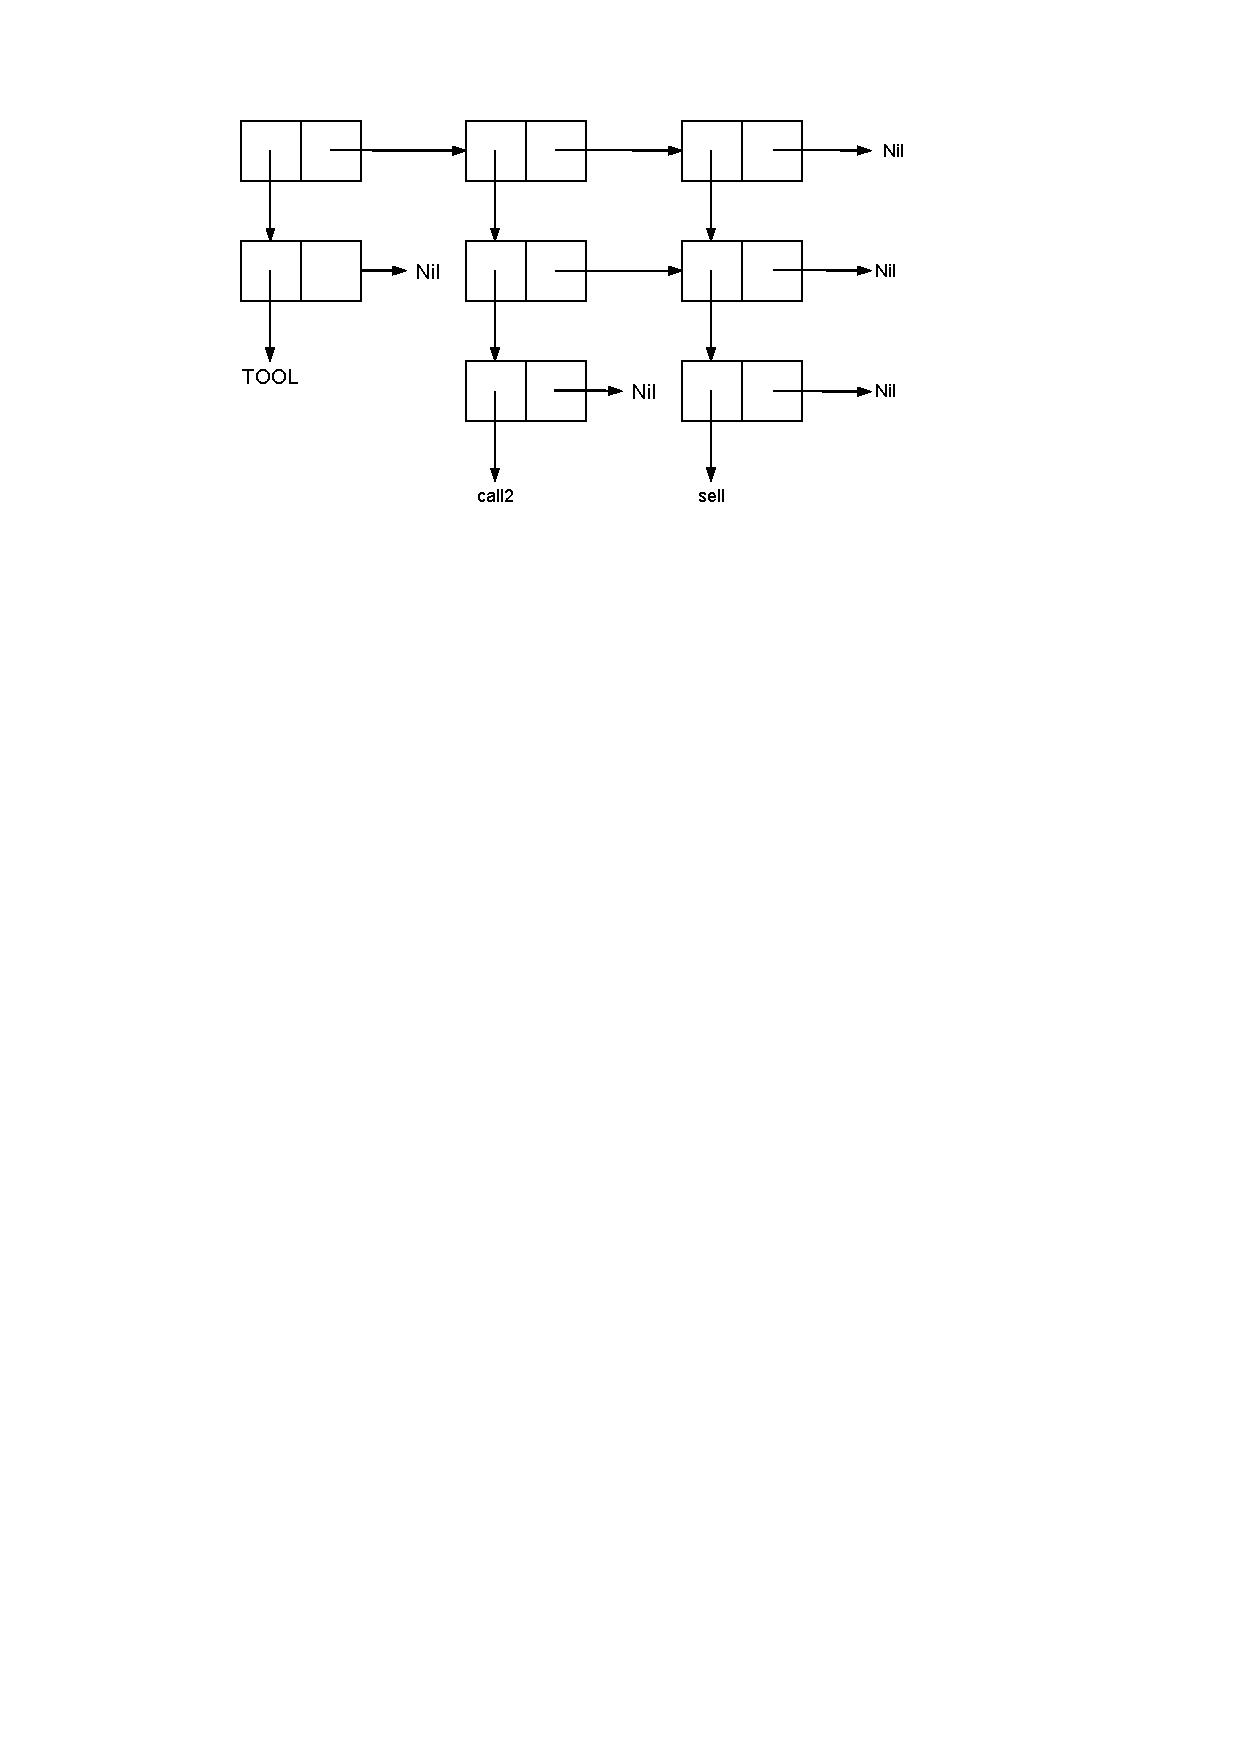
\includegraphics[scale=1]{images/task_1 (5).pdf}}
\end{figure} 

'(((TOOL) (call)) ((sell)))
\begin{figure}[H]
	\centering{
		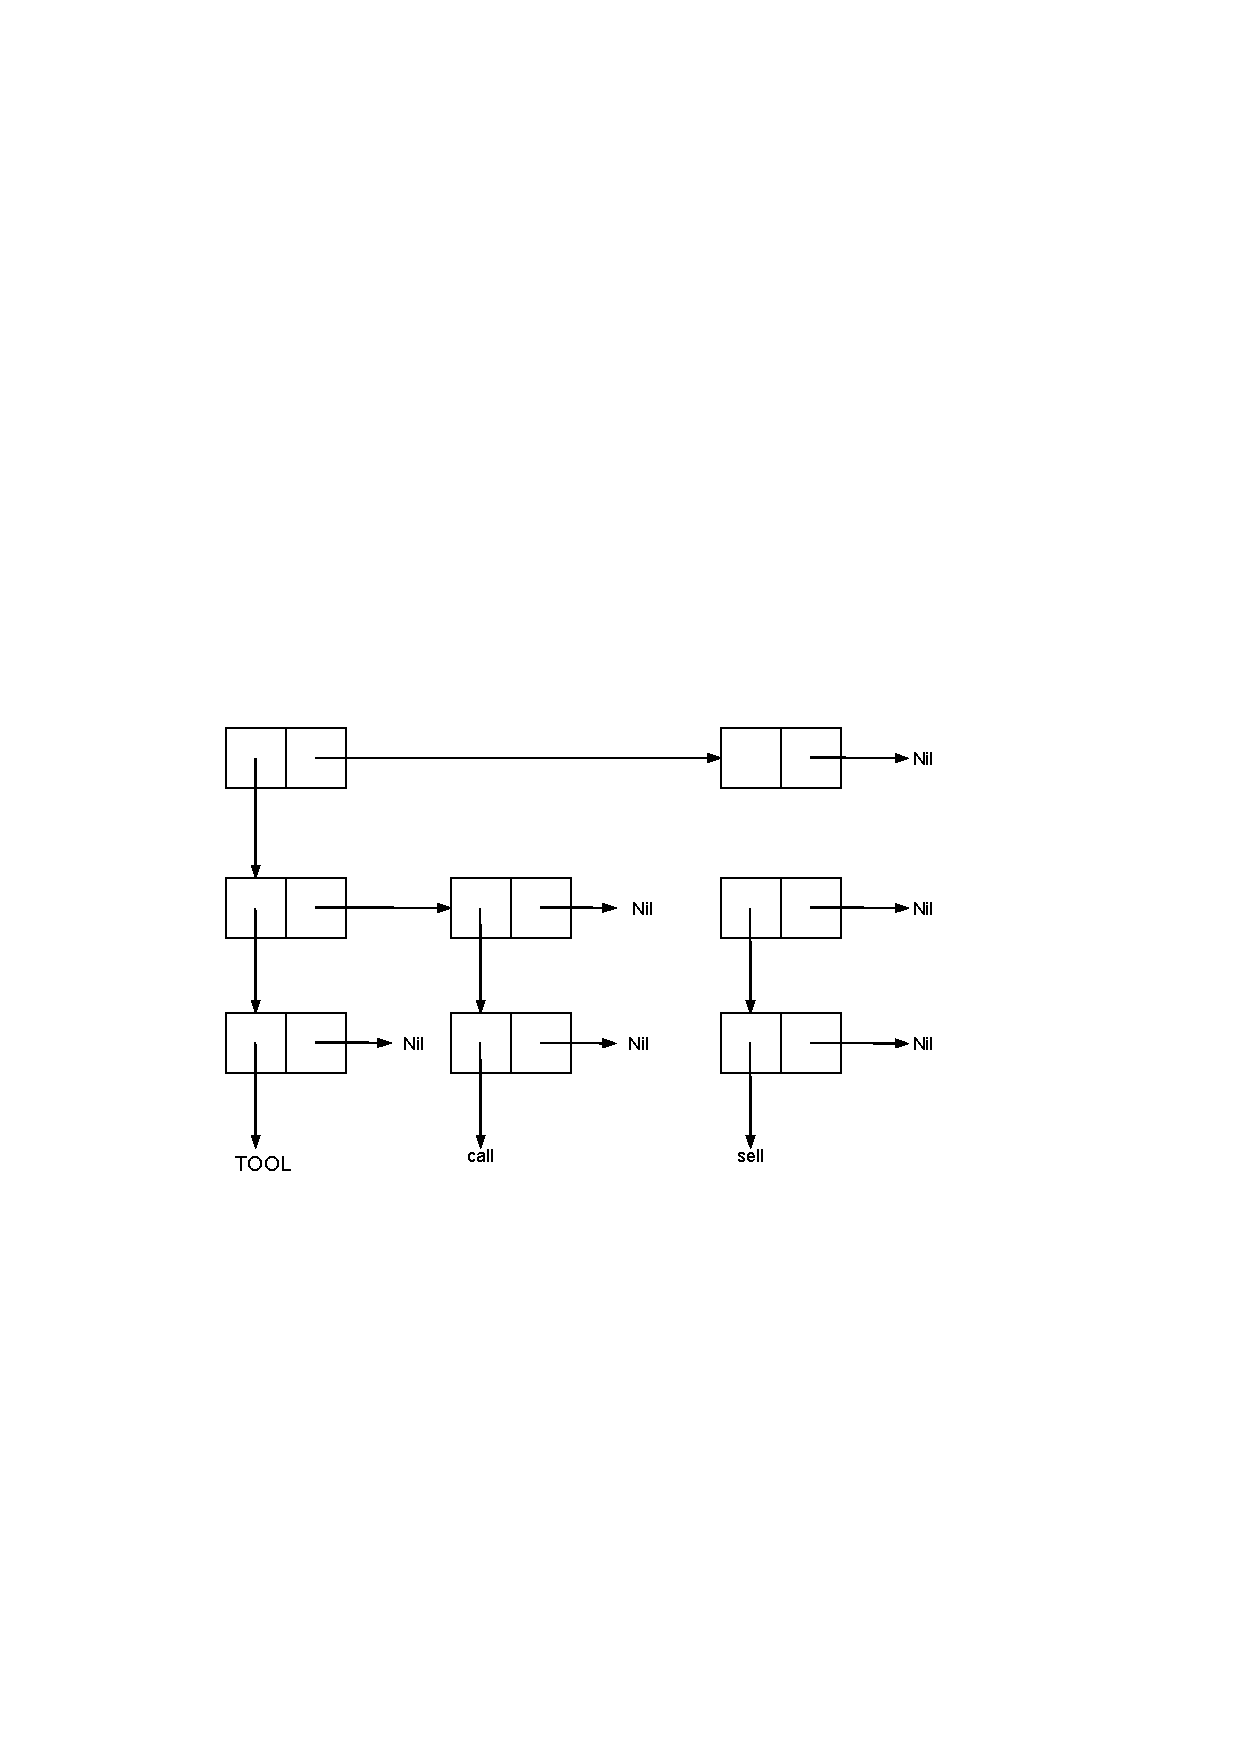
\includegraphics[scale=1]{images/task_1 (6).pdf}}
	\end{figure} 

\section{Использующие только функции CAR и CDR, написать выражения, возвращающие второй, третий, четвертый элементы заданного списка}

\begin{enumerate}
	\item второй элемент: (car (cdr '(a b c d e f)))
	\item третий элемент: (car (cdr (cdr '(a b c d e f))))
	\item четвертый элемент: (car (cdr (cdr (cdr '(a b c d e f)))))
\end{enumerate}

\section{Что будет в результате вычисления выражений?}
\begin{enumerate}
	\item[a)] (CAADR '((blue cube) (red pyramid)))
	
	(car (car (cdr '((blue cube) (red pyramid)))))
	
	(car (car '(red pyramid)))
	
	(car '(red)) => red
	
	\item[b)] (CDAR '((abc) (def) (ghi)))
	
	(cdr (car '((abc) (def) (ghi))))
	
	(cdr '((abc)) => Nil
	
	\item[c)] (CADR '((abc) (def) (ghi)))
	
	(car (cdr '((abc) (def) (ghi))))
	
	(car '((def) (ghi))) => (def)
	 
	\item[d)]  (CADDR '((abc) (def) (ghi)))
	
	(car (cdr (cdr '((abc) (def) (ghi)))))
	
	(car (cdr '((def) (ghi))))
	
	(car '((ghi))) => (ghi)
\end{enumerate}

\section{Напишите результат вычисления выражений и объясните, как он получен}
\begin{enumerate}
	\item (list 'Fred 'and 'Wilma)
	
	(cons 'Fred (cons 'and (cons 'Wilma ())))
	
	(Fred and Wilma)
	
	\item (list 'Fred '(and Wilma))
	
	(cons 'Fred (cons '(and Wilma) ()))
	
	(cons 'Fred (and Wilma))
	
	(Fred (and Wilma))
	
	\item (cons Nil Nil) => (Nil)
	
	\item (cons T Nil) => (T)
	\item (cons Nil T) => (Nil.T)
	\item (list Nil)
	
	(cons Nil Nil) => (Nil)
		
	\item (cons '(T) Nil) => ((T))
	
	\item (list '(one two) '(free temp))
	
	(cons '(one two) (cons '(free temp) ()))
	
	((one two) (free temp))
	
	\item (cons 'Fred '(and Wilma))
	
	(Fred and Wilma)
	
	\item (cons 'Fred '(Wilma))
	
	(Fred Wilma)
	
	\item (list Nil Nil)
	
	(cons Nil (cons Nil Nil)) => (Nil Nil)
	
	\item (list T Nil)
	
	(cons T (cons (Nil Nil)) => (T Nil)
	
	\item (list Nil T)
	
	(cons Nil (cons T Nil)) => (Nil T)
	
	\item (cons T (list Nil))
	
	(cons T (cons Nil Nil))
	
	(cons T Nil) 
	
	(T)
	
	\item (list '(T) Nil)
	
	((T) Nil)
	
	\item (cons '(one two) '(free temp))
	
	((one two) free temp)	
\end{enumerate}

\section{Написать лямбда-выражение и соответствующую функцию. Представить результаты в виде списочных ячеек.}
\begin{itemize}
	\item Написать функцию (f ar1 ar2 ar3 ar4), возвращающую список 
	
	((ar1 ar2) (ar3 ar4)).
	
	(defun f (ar1 ar2 ar3 ar4) (cons '(ar1 ar2) (cons '(ar3 ar4) ())))
	
	\begin{figure}[H]
		\centering{
			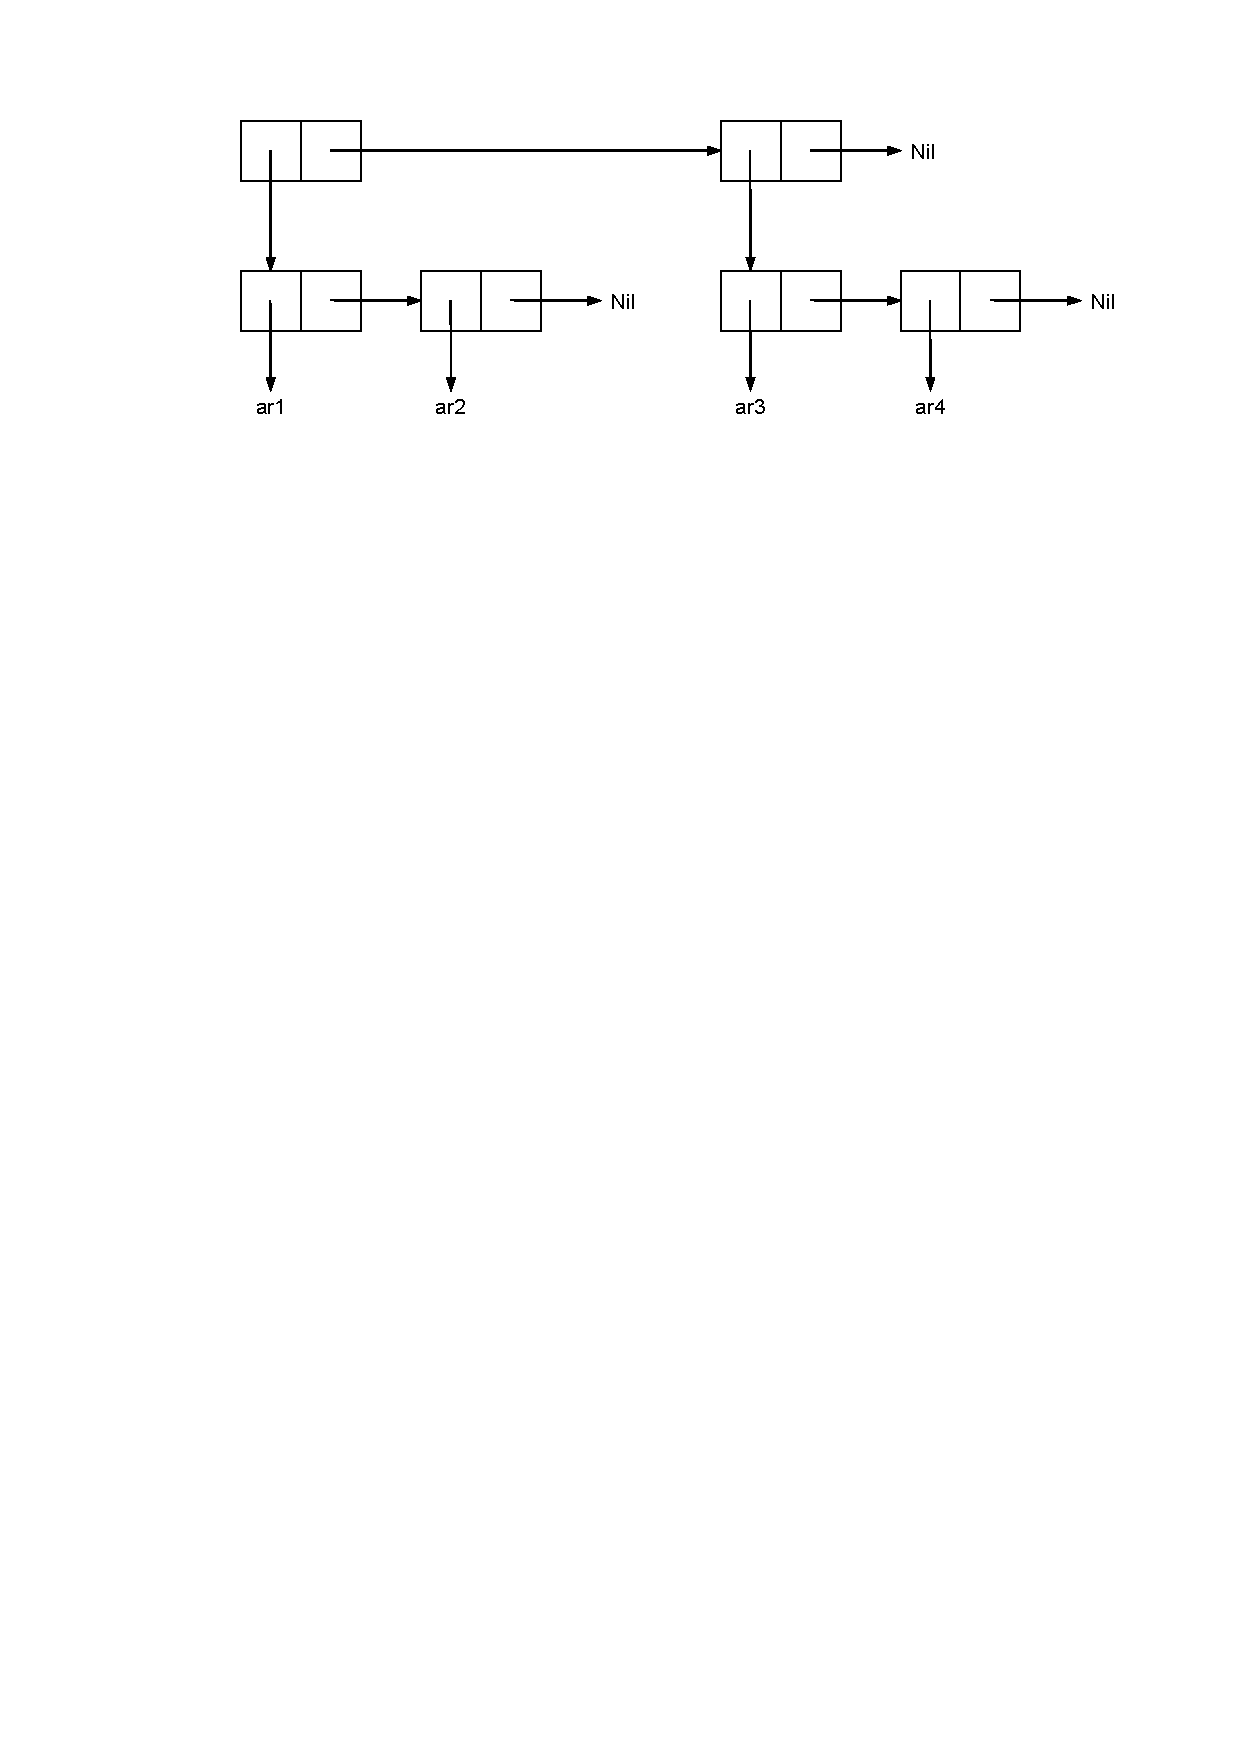
\includegraphics[scale=1]{images/task_5_1.pdf}}
	\end{figure} 
	
	\item Написать функцию (f ar1 ar2), возвращающую ((ar1) (ar2)).
	
	(defun f (ar1 ar2) (cons '(ar1) (cons '(ar2) ())))
	
	\begin{figure}[H]
		\centering{
			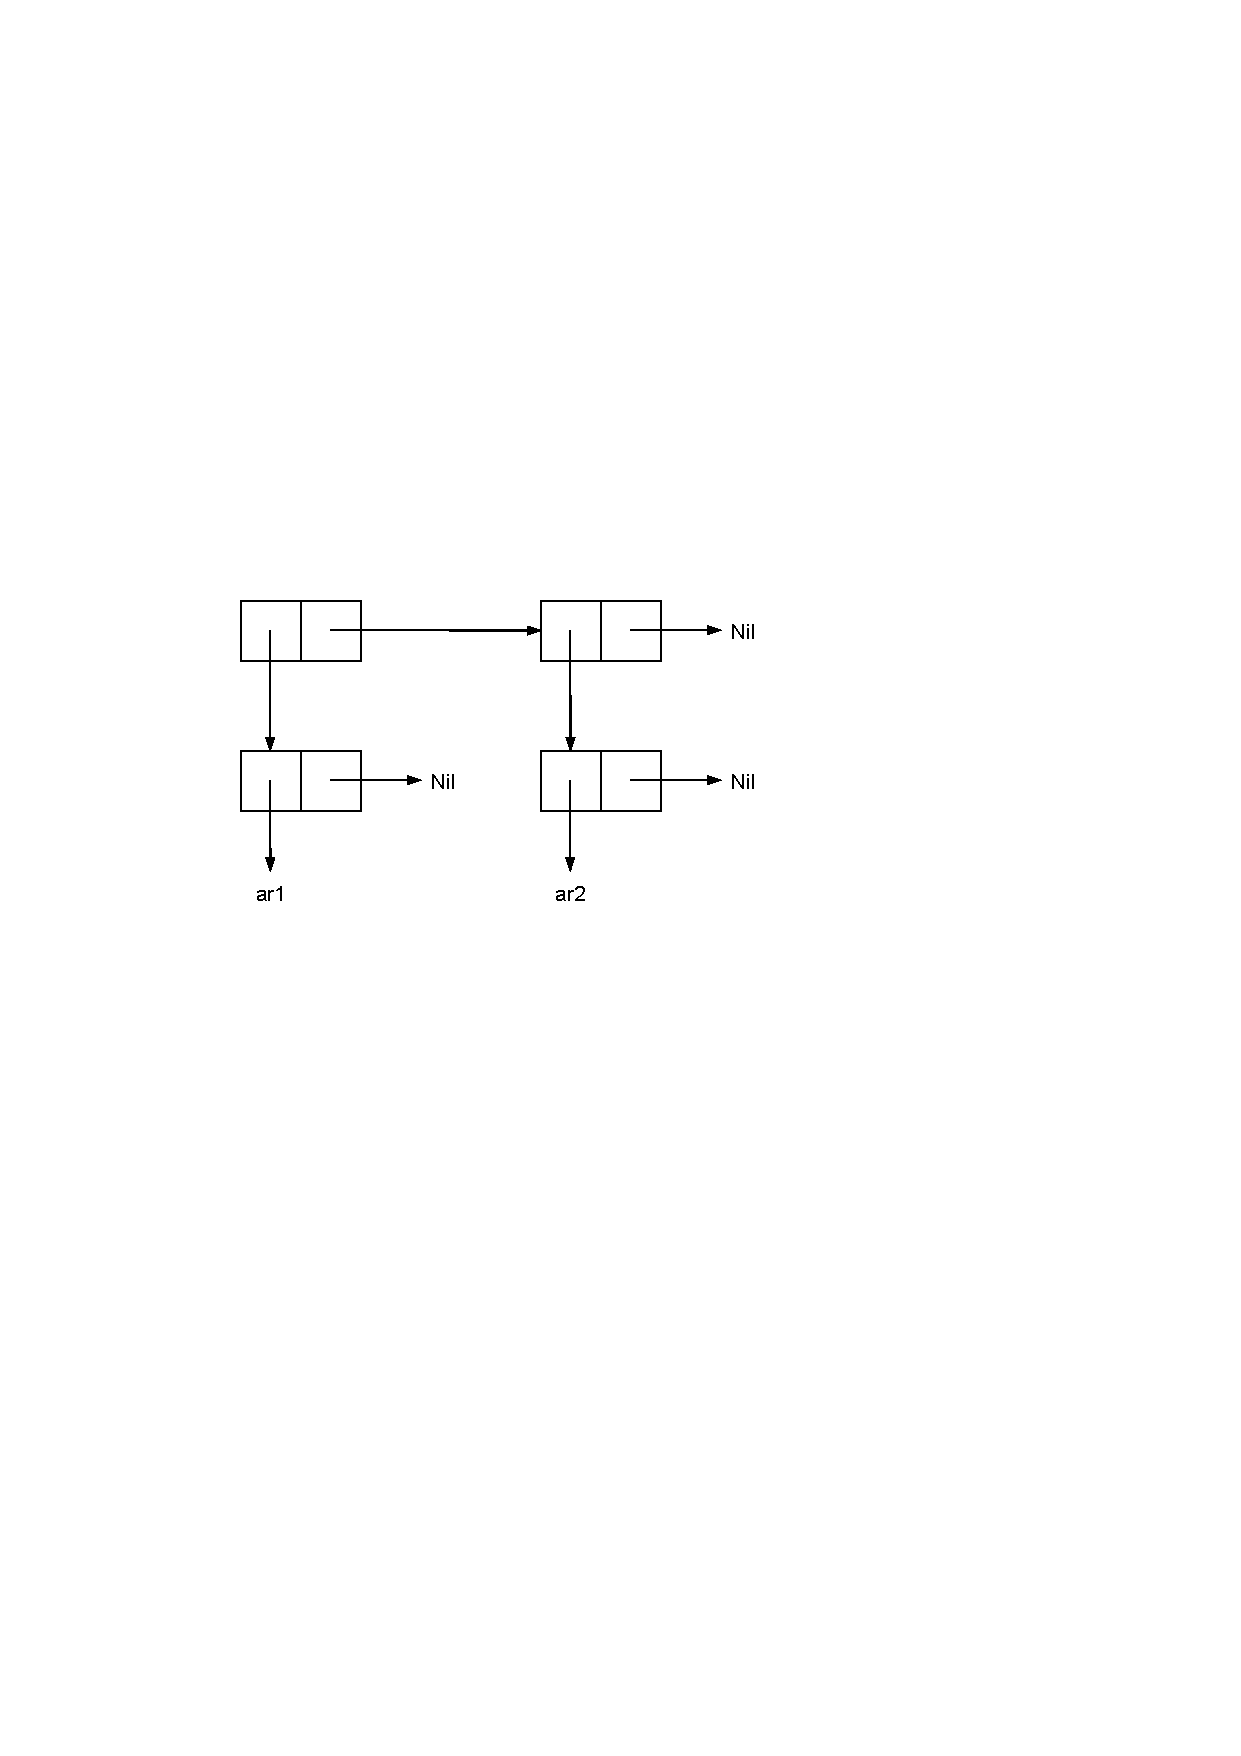
\includegraphics[scale=1]{images/task_5_2.pdf}}
	\end{figure} 
	
	\item Написать функцию (f ar1), возвращающую (((ar1))).
	
	(defun f (ar1) (cons (cons '(ar1) ()) ()))
	
	\begin{figure}[H]
		\centering{
			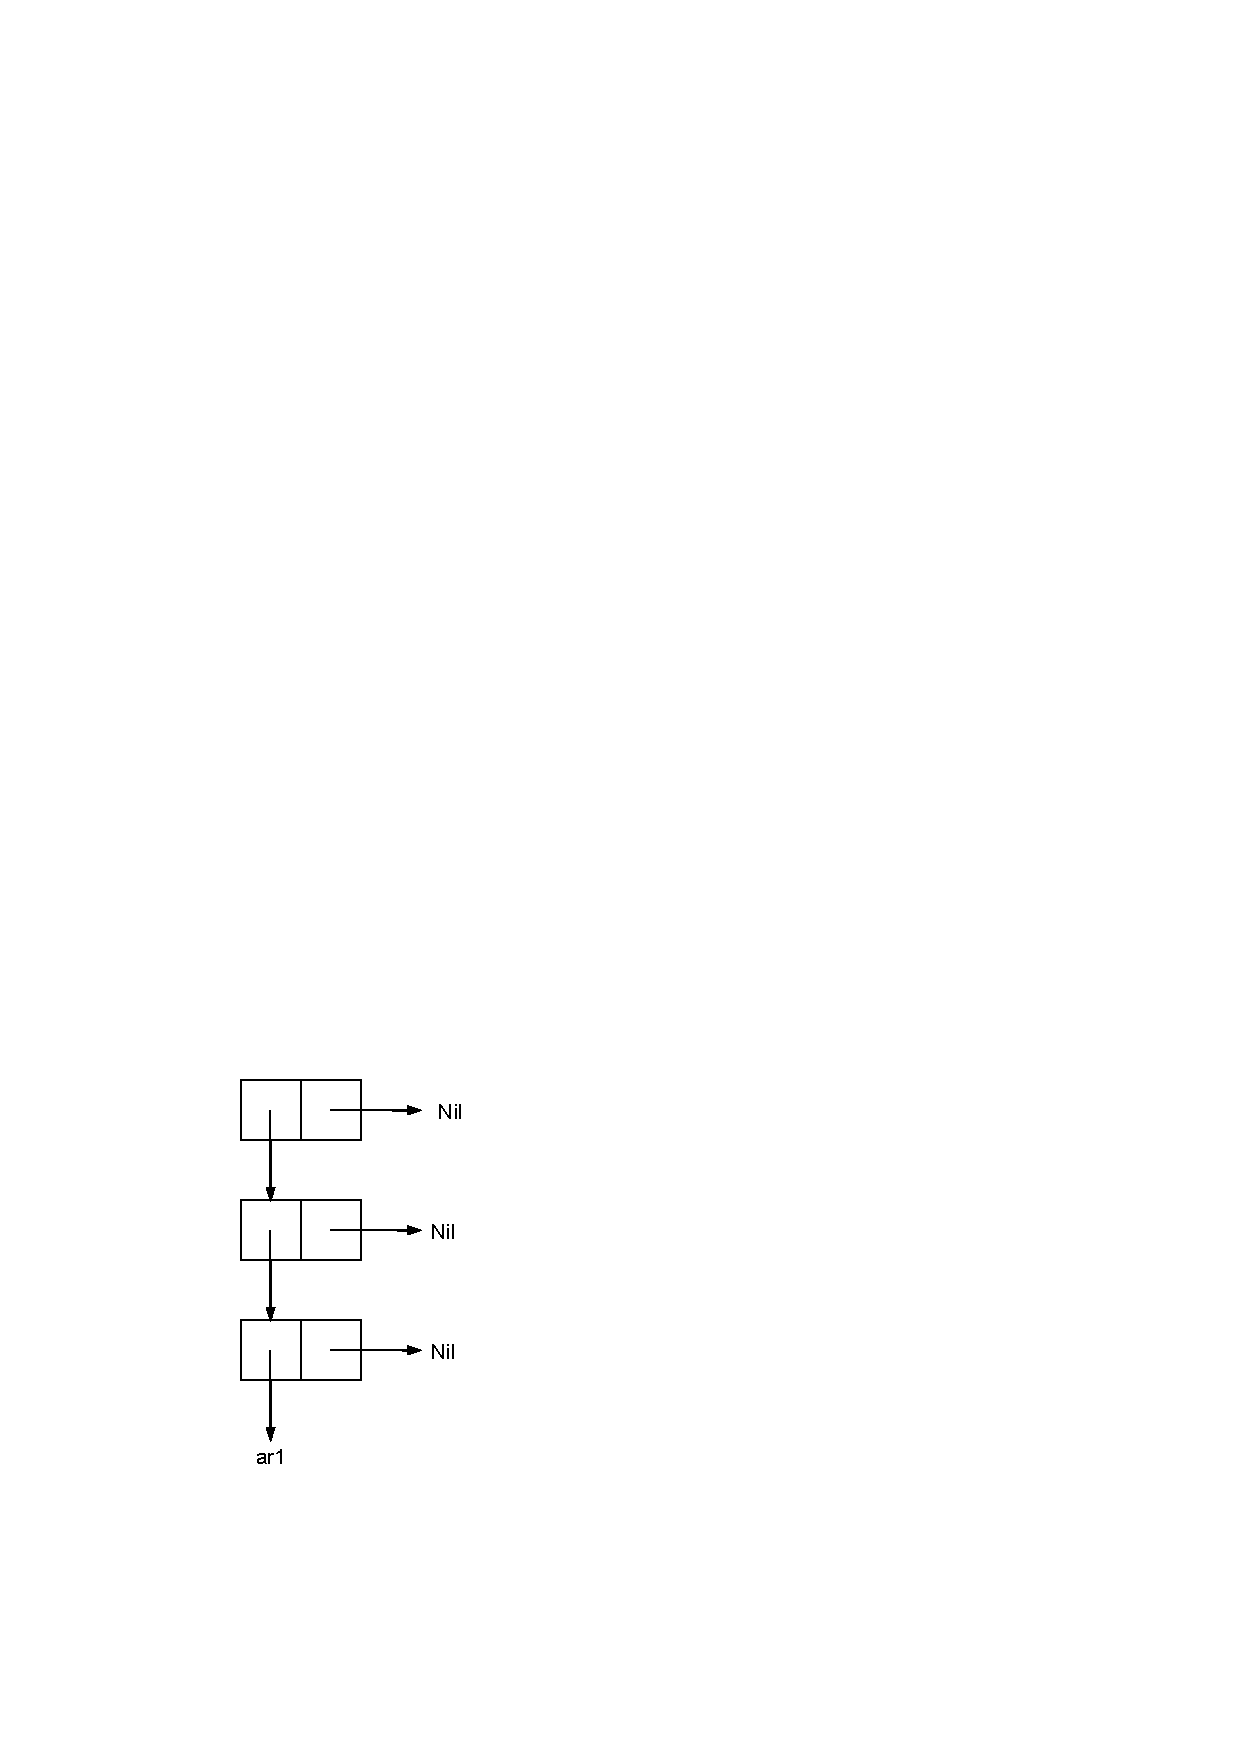
\includegraphics[scale=1]{images/task_5_3.pdf}}
	\end{figure} 
\end{itemize}